\documentclass[11pt]{article}
\usepackage[czech]{babel}
\usepackage[T1]{fontenc}
\usepackage{xcolor}
\usepackage{listings}
\usepackage{indentfirst}
\usepackage{amsmath}
\usepackage{amssymb}
\usepackage{hyperref}
\usepackage{graphicx}
\usepackage{mathtools}
\DeclarePairedDelimiter{\abs}{\lvert}{\rvert}
\graphicspath{ {./images/} }


\definecolor{codegreen}{rgb}{0,0.6,0}
\definecolor{codegray}{rgb}{0.5,0.5,0.5}
\definecolor{codepurple}{rgb}{0.58,0,0.82}
\definecolor{backcolour}{rgb}{0.95,0.95,0.92}

\lstdefinestyle{mystyle}{
    backgroundcolor=\color{backcolour},   
    commentstyle=\color{codegreen},
    keywordstyle=\color{magenta},
    numberstyle=\tiny\color{codegray},
    stringstyle=\color{codepurple},
    basicstyle=\ttfamily\footnotesize,
    breakatwhitespace=false,         
    breaklines=true,                 
    captionpos=b,                    
    keepspaces=true,                 
    numbers=left,                    
    numbersep=5pt,                  
    showspaces=false,                
    showstringspaces=false,
    showtabs=false,                  
    tabsize=2
}

\lstset{style=mystyle}

\title{Dlouhodoba maturitni prace \\
\large Teoreticky rozebrat a popsat shorův kvantový algoritmus na lámání šifry RSA. Implementovat algoritmus v nějakém simulátoru a použít ho na prolomení RSA s malým modulusem}

\author{Dmitry Leshchinskiy}
\date{\today}

\begin{document}
\maketitle
\newpage

\tableofcontents
\newpage

\section{Uvod do RSA}
\subsection{Co je to RSA?}

RSA je asymetricka sifra s otevrenym klicem. Pro pouziti teto sifry je potreba si vypocitat otevreny klic, kterym se bude sifrovat zprava urcena pro vas, a privatni klic, kterym vy budete sifru desifrovat. K aktualnimu dni se tato sifra povazuje za bezpecnou.

\subsection{Princip RSA}
Kdyz budu chtit nekomu poslat zakodovanou zpravu pomoci RSA, potrebuju si od adresata dostat jeho verejny klic. Timto klicem si zkoduju zpravu a odeslu mu ji zpet. Prijemce az zpravu dostane, desifruje ji pomoci sveho privatniho klice.
\par Bezpecnost RSA je postavena na predpokladu, ze je dost narocne faktorizovat cislo. Faktorizovat cislo znamena rozlozit jej na soucin prvocisel.

\subsection{Vypocet klicu teorie}
Nejdriv si osoba musi vybrat dve prvocisla $p, q$.
Nasledne se vypocita jejich nasobek. Oznacime ho za $N$.
Dale si nadefinujem $\phi (N)$ jako $(p - 1) * (q - 1)$.
\par V následujícím kroku se musí vybrat číslo $e$, pro které plati, ze je nesoudelne s $\phi (N)$.
Pro nalezeni $e$ lze vyuzit rozsireny Eukliduv algoritmus.
Poslednim krokem je urcit číslo $d$. Pro d plati:
$$ ed \bmod \phi (N) = 1 $$
Verejny klic je pak dvojice: $e, N$ \\
Privatni klic je pak dvojice: $d, N$

\subsection{Vypocet klicu ukazka}
\noindent Zvolime si nejprve $p, q$:
$$p = 83, q = 89$$
Spocitam $N, \phi (N)$:
$$N = pq = 83 * 89 = 7387$$
$$\phi (N) = (p - 1)(q - 1) = 82 * 88 = 7216$$
Ziskam $e, d$:
$$e = 3 \because gcd(e, \phi (N)) = 1$$
$$d = 4811 \because ed \bmod \phi (N) = 1$$
Poskladam klice:
Public: $(3, 7387)$
Private: $(4811, 7387)$


\subsection{Sifrovani a desifrovani}
Nejdriv si popisem sifrovani.
Mejme zpravu m a public klic $(e, N)$. Pak se zprava zasifruje do $c$ nasledovne:
$$c = m^e \bmod N$$
Proto abychm mohli zprávy dešifrovat, potrénujeme privatni klic. Pak se zprava $c$ desefruje pomoci privátního klice $(d, N)$ do $m$ nasledne:
$$m = c^d \bmod N$$
Vsime me si, ze muze docházet k umocneni velkou exponentou.

\subsection{Prolomeni RSA}
Jak jiz bylo zmineno, RSA se povazuje za bezpečnou sifru. Na venek je prestupna jen zasifrovana zprava c a verejny klic (e, N), který byla zprava zasifrovana.

\par Pro desifrovani potrebujem privatni klic $(d, N)$.
Pro vypocet $d$ potrebujem si dopočítat $\phi (N)$, který se pocita z $p$ a $q$.
Nastesti nebo k nestesti, zalezi na pohledu, zname $N$, coz je soucin $p$ a $q$.
Takze potrebujem jen rozlozit $N$ na soucin dvou prvočísel neboli faktorizovat.

\par Zatim neexistuje zadny algoritmus pro faktorizaci, který by bezel na klasickem pocitaci za polynomialni cas.
Avsak v roce 1994 se podarilo P. Shorovi, americkému profesorovi matematiky v MIT, vymyslet algorithmus, který by bezel castecne na kvantovem pocitaci, a výsledkem je rozlozene číslo na soucin prvočísel.
Ten algoritmus si pojmenoval jako Shoruv algoritmus.[\url{https://arxiv.org/pdf/quant-ph/9508027.pdf}]


\newpage

\section{Uvod do Kvantovych pocitacu}
\subsection{Co je kvantovy pocitac?}
Kvantovy pocitac je teoriticky model zarizeni pro vypocty.
Primo vyuziva fenomény z kvantove mechaniky jako superpozice nebo interference.
Zatím co klasicky pocitac operuje s bity, kvantovy pocitac operuje s qubity.
Jednotlivym skupinam qubitu se říká registr.

\subsection{Co je to Qubit?}
Klasicky bit v pocitaci muze nabývat hodnot ${0, 1}$. Qubit muze byt $0$, $1$ nebo kombinaci obou. Da se zapsat jako vektor:
$$|q\rangle = \alpha|0\rangle + \beta|1\rangle$$
\par kde $\alpha$ a $\beta$ jsou koeficienty, které urcuji pravdepodobnost změřeni qubitu ve stavu $0$ nebo $1$.
Soucet druhých mocnin koeficientu se musí rovnat $1$:
$$\alpha^2 + \beta^2 = 1$$
\par Zapis $|0\rangle$ a $|1\rangle$ neni nic jiného nez jenom zkraceny zapis vektoru.
Muzeme to tedy rozepsat takto:
$$|0\rangle = \begin{bmatrix}
        1 \\
        0
    \end{bmatrix} |1\rangle = \begin{bmatrix}
        0 \\
        1
    \end{bmatrix}  $$
\par Muzem tedy upravit a prepsat stav qubitu $|q\rangle$ jako:
$$|q\rangle = \begin{bmatrix}
        \alpha \\
        \beta
    \end{bmatrix}$$

\par Ukazeme si, jak matematicky funguje mereni.
Proto abychom zjistili pravdepodobnost pro konkretni stav, nam staci umocnit na druhou násobek transpozovane matice hledaneho stavu a matici $|q\rangle$:
$$|\langle 0 | q \rangle|^2 = \abs*{\begin{bmatrix}
            1 & 0
        \end{bmatrix}\begin{bmatrix}
            \alpha \\
            \beta
        \end{bmatrix}}^2 = \alpha ^ 2$$

$$|\langle 1 | q \rangle|^2 = \abs*{\begin{bmatrix}
            0 & 1
        \end{bmatrix}\begin{bmatrix}
            \alpha \\
            \beta
        \end{bmatrix}}^2 = \beta ^ 2$$




\subsection{Registr Qubitu}
Ve výpočtech většinou nebudeme pracovat s jednym qubitem ale s celym registrem qubitu. Zkraceny zapis by vypadal takto:
$$|001\rangle$$
\par To znamena, ze mam 3 qubity, první 2 jsou nastavene na 0, poslední je nastaven na 1.
Když budeme chtit si to představit jako vektor, staci zjiskat kronekeruv soucin:
$$|q\rangle = |001\rangle = |0\rangle \otimes |0\rangle \otimes |1\rangle = \begin{bmatrix}
        0 \\
        1 \\
        0 \\
        0 \\
        0 \\
        0 \\
        0 \\
        0 \\
    \end{bmatrix}$$
\par Pravidla pro mereni funguji stejne:
$$|\langle001|q\rangle|^2 = 1$$
$$|\langle 011|q\rangle|^2 = 0$$


\subsection{Kvantove hradlo}
V booleve algebre mame logicke ventily typu OR, AND, XOR. To jsou ventily, které dostavaji vstup bitu a produkuji vystup. Kvantove pocitace mají něco podobneho. Nejvetsi rozdil je v tom, ze kvantove ventily provádí jenom reverzibilni operace.
Všechna kvantova hradla jsou reverzibilni. To znamena, ze kdybychom aplikovali dve hradla za sebou, budeme mit na vystupu druhého hradla presne to, co jsme meli na vstupu prvního hradla.
\par Každý hradlo je matematicky definovano čtvercovou matici o rozmerech $2^n \times 2^n$, kde $n$ je počet qubitu. Pro aplikovani hradla je potřeba vynásobit mezi sebou matici hradla a vektor stavu $|q\rangle$.
\par Zakladni kvantove hradlo je \textbf{I} jako identita. Presneji receno nedela nic ale i tak bude potřeba pro nektere vypocty. Jeji matice vypada takto:
$$I = \begin{bmatrix}
        1 & 0 \\
        0 & 1
    \end{bmatrix}$$
\par Nejjednodussi reverzibilni hradlo v klasickem pocitaci je NOT.
Provadi negaci bitu. V kvantovem svete existuje podobny hradlo, které také neguje hodnotu.
Presneji receno otaci  Blochovou kouli podle $x$ osy o $\pi$ radianu. Znaci se jako \textbf{X} gate.
Jeho matice je nasledujici:
$$X = \begin{bmatrix}
        0 & 1 \\
        1 & 0
    \end{bmatrix}$$
\par Jako dukaz, ze se jedna o hradlo reverzibilni, muzem zkusit je poskládat za sebou a podivat se co nam vyjde.
To znamena, ze je vynasobime mezi sebou:
$$XX = \begin{bmatrix}
        0 & 1 \\
        1 & 0
    \end{bmatrix}\begin{bmatrix}
        0 & 1 \\
        1 & 0
    \end{bmatrix} = \begin{bmatrix}
        1 & 0 \\
        0 & 1
    \end{bmatrix} = I$$

\par Ve vysledku mame hradlo \textbf{I}, které jak vime nedela nic s vektorem stavu $|q\rangle$.
\par Dalsim hodne zajimavym hradlem, který bude potřeba pro Shoruv algorithmus je Hadamard gate, který se znaci \textbf{H}. Jeho matice:
$$H = \frac{1}{\sqrt{2}}\begin{bmatrix}
        1 & 1  \\
        1 & -1
    \end{bmatrix}$$
\par Toto hradlo prevadi qubit do stavu superpozice. Dulezite je zminit, ze superpozice vytvorena z qubitu ve stavu 0, se bude vyrazne lisit od superpozice vytvorene z qubitu ve stavu 1.
Tady je vypocet:
$$H|0\rangle = \frac{1}{\sqrt{2}}\begin{bmatrix}
        1 & 1  \\
        1 & -1
    \end{bmatrix}\begin{bmatrix}
        1 \\
        0
    \end{bmatrix} = \frac{1}{\sqrt{2}}\begin{bmatrix}
        1 \\
        1
    \end{bmatrix} = \frac{|0\rangle + |1\rangle}{\sqrt{2}} = |+\rangle$$

$$H|1\rangle = \frac{1}{\sqrt{2}}\begin{bmatrix}
        1 & 1  \\
        1 & -1
    \end{bmatrix}\begin{bmatrix}
        0 \\
        1
    \end{bmatrix} = \frac{1}{\sqrt{2}}\begin{bmatrix}
        1 \\
        -1
    \end{bmatrix} = \frac{|0\rangle - |1\rangle}{\sqrt{2}} = |-\rangle$$

\par Vsimne te si, ze rozdil je pouze v znamenku u koeficientu $\beta$. Proto první superpozice se oznacuje jako $|+\rangle$ a druha jako $|-\rangle$.
Zajimavy je, ze když provedem mereni stavu superpozice, vyjde nam, ze je $\frac{1}{2}$ sance, ze qubit bude ve stavu 0 a stejna sance, ze bude ve stavu 1.


\subsection{Ventily s kontrolním qubitem}
Existuje další typ hradel, kterym se anglicky říká Control gates.
Chovani těchto hradel je zavisle na jakemsi kontrolním qubitu.
Nejznamejsi pripad je CNOT neboli Controlled NOT. Matice hradla je:
$$CNOT = \begin{bmatrix}
        1 & 0 & 0 & 0 \\
        0 & 1 & 0 & 0 \\
        0 & 0 & 0 & 1 \\
        0 & 0 & 1 & 0
    \end{bmatrix}$$
\par Toto hradlo dostava na vstupu dva qubity.
Zde dochazi k invertaci v pripade, ze je první qubit ve stavu 1.
Jinak se nedeje nic. Par prikladu:
$$CNOT|01\rangle = \begin{bmatrix}
        1 & 0 & 0 & 0 \\
        0 & 1 & 0 & 0 \\
        0 & 0 & 0 & 1 \\
        0 & 0 & 1 & 0
    \end{bmatrix}\begin{bmatrix}
        0 \\
        1 \\
        0 \\
        0
    \end{bmatrix} = \begin{bmatrix}
        0 \\
        1 \\
        0 \\
        0
    \end{bmatrix} = |01\rangle$$

$$CNOT|11\rangle = \begin{bmatrix}
        1 & 0 & 0 & 0 \\
        0 & 1 & 0 & 0 \\
        0 & 0 & 0 & 1 \\
        0 & 0 & 1 & 0
    \end{bmatrix}\begin{bmatrix}
        0 \\
        0 \\
        0 \\
        1
    \end{bmatrix} = \begin{bmatrix}
        0 \\
        0 \\
        1 \\
        0
    \end{bmatrix} = |10\rangle$$

\par Je mozne poskládat matici pro libovolny kontrolni hradlo. Ukazu to na prikladu CNOTu.
$$CNOT = |1 \rangle\langle 1| \otimes X + |0 \rangle\langle 0| \otimes I$$
$$CNOT = \begin{bmatrix}
        0 \\
        1
    \end{bmatrix}\begin{bmatrix}
        0 & 1
    \end{bmatrix} \otimes \begin{bmatrix}
        0 & 1 \\
        1 & 0
    \end{bmatrix} + \begin{bmatrix}
        1 \\
        0
    \end{bmatrix}\begin{bmatrix}
        1 & 0
    \end{bmatrix} \otimes \begin{bmatrix}
        1 & 0 \\
        0 & 1
    \end{bmatrix}$$
$$CNOT = \begin{bmatrix}
        0 & 0 & 0 & 0 \\
        0 & 0 & 0 & 0 \\
        0 & 0 & 0 & 1 \\
        0 & 0 & 1 & 0
    \end{bmatrix} + \begin{bmatrix}
        1 & 0 & 0 & 0 \\
        0 & 1 & 0 & 0 \\
        0 & 0 & 0 & 0 \\
        0 & 0 & 0 & 0
    \end{bmatrix} = \begin{bmatrix}
        1 & 0 & 0 & 0 \\
        0 & 1 & 0 & 0 \\
        0 & 0 & 0 & 1 \\
        0 & 0 & 1 & 0
    \end{bmatrix}$$

\subsection{Vzajemne spoutane qubity – Bellmanuv Stav}
Myslim si, ze je dost jasne jak se budou chovat 2 qubity po CNOTu.
Control qubit zustane stejny ale druhy(target) qubit se zmeni pokud je první ve stavu 1.
Co se však stane, když controlni qubit bude v superpozici? Pojdme si to spočítat.
Budeme mit tenhle pocatecni stav:
$$|\phi_1 \rangle = |00\rangle = \begin{bmatrix}
        1 \\
        0 \\
        0 \\
        0
    \end{bmatrix}$$
\par Proto abychom dostali stav superpozice, potrebujem ventil Hadamarda.
V nasem pripade bude první qubit kontrolni, takze potrebujem aplikovat Hadamarda na první qubit:
$$|\phi_2 \rangle = (H \otimes I) |\phi_1 \rangle = \frac{1}{\sqrt{2}} \begin{bmatrix}
        1 & 0 & 1  & 0  \\
        0 & 1 & 0  & 1  \\
        1 & 0 & -1 & 0  \\
        0 & 1 & 0  & -1
    \end{bmatrix}\begin{bmatrix}
        1 \\
        0 \\
        0 \\
        0
    \end{bmatrix} = \frac{1}{\sqrt{2}}\begin{bmatrix}
        1 \\
        0 \\
        1 \\
        0
    \end{bmatrix}$$
\par Tento stav nam říká, ze je mozny po zmereni dostat bud $|00\rangle$ nebo $|10\rangle$ s $\frac{1}{2}$ pravdepodobnosti.
Nasledne pojdme aplikovat CNOT:
$$|\phi_3 \rangle = CNOT |\phi_2 \rangle = \frac{1}{\sqrt{2}} \begin{bmatrix}
        1 & 0 & 0 & 0 \\
        0 & 1 & 0 & 0 \\
        0 & 0 & 0 & 1 \\
        0 & 0 & 1 & 0
    \end{bmatrix}\begin{bmatrix}
        1 \\
        0 \\
        1 \\
        0
    \end{bmatrix} = \frac{1}{\sqrt{2}}\begin{bmatrix}
        1 \\
        0 \\
        0 \\
        1
    \end{bmatrix}$$
\par Timto jsme dostali Belluv stav, při nemz jsou 2 qubity spolecne spoutany.
Ted když provedem mereni, dostanem bud $|00\rangle$ nebo $|11\rangle$ s $\frac{1}{2}$ pravdepodobnosti.
Tento stav se pouziva u algorithmu kvantove teleportace.

\subsection{Phase kick-back}
Pojdme si podivat, co se stane, kdy aplikujem \textbf{X} gate na stav $|+\rangle$ nebo $|-\rangle$:
$$X|+\rangle = \frac{1}{\sqrt{2}}\begin{bmatrix}
        0 & 1 \\
        1 & 0
    \end{bmatrix} + \begin{bmatrix}
        1 \\
        1
    \end{bmatrix} = \frac{1}{\sqrt{2}} \begin{bmatrix}
        1 \\
        1
    \end{bmatrix} $$

$$X|-\rangle = \frac{1}{\sqrt{2}}\begin{bmatrix}
        0 & 1 \\
        1 & 0
    \end{bmatrix} + \begin{bmatrix}
        1 \\
        -1
    \end{bmatrix} = \frac{1}{\sqrt{2}} \begin{bmatrix}
        -1 \\
        1
    \end{bmatrix} = -\frac{1}{\sqrt{2}} \begin{bmatrix}
        1 \\
        -1
    \end{bmatrix} $$
\par Na první pohled nic moc překvapivého.
Ale jedna se o první krok k porozumeni důležitého konceptu: phase kick-back.
Drive jsme si mysleli, ze při pouziti CNOTu, ovlivnujem pouze cilovy qubit.
Ale ted si ukazem, ze ovlivnujem i kontrolni.
Pro demonstraci je potřeba CNOT aplikovat na cilovy qubit ve stavu superpozice.
Nejdriv pro kontrolni ve stavu $|0\rangle$, nasledne ve stavu $|1\rangle$:
$$CNOT |0-\rangle = |0\rangle \left(\frac{|0\rangle - |1\rangle}{\sqrt{2}}\right)$$
$$CNOT |1-\rangle = |1\rangle \left(X \left(\frac{|0\rangle - |1\rangle}{\sqrt{2}}\right)\right) = |1\rangle \left(-1\left(\frac{|0\rangle - |1\rangle}{\sqrt{2}}\right)\right) =$$
$$= -|1\rangle \left(\frac{|0\rangle - |1\rangle}{\sqrt{2}}\right)$$
\par Obecne plati:
$$CNOT |b-\rangle = (-1)^b|b\rangle\left(\frac{|0\rangle - |1\rangle}{\sqrt{2}}\right)$$:
\par Je videt, ze jsme dokazali zmenit fazi kontrolního qubitu, když kontrolni qubit je v superpozici:
$$CNOT\left((\alpha|0\rangle + \beta|1\rangle)\left(\frac{|0\rangle - |1\rangle}{\sqrt{2}}\right)\right) = (\alpha|0\rangle - \beta|1\rangle)\left(\frac{|0\rangle - |1\rangle}{\sqrt{2}}\right)$$
\newpage

\section{QuantumEmulator – vlastni kvantovy simuator}
\subsection{Uvod}
QuantumEmulator – je moje vlastní Python knihovna, která mi pomáhala ve zkoumani funkcnosti kvantového pocitace.
Nabizi funkce pro tvorbu kvantových algoritmu libovolne slozitosti.
\par Jelikoz simulace kvantového pocitace je hodne o pocitani s maticemi, vybral jsem si knihovnu Numpy, která zjednodusuje praci s maticemi a celkove s vypocty.
Numpy vyuziva funkce psane v jazyce C, a proto jsou vypocty optimalizovane.
\par Projekt je pod licenzi MIT a lze ho najit na mem githubu zde: \url{https://github.com/DimaLeshchinskiy/QuantumEmulator}

\subsection{QConstants}
Tento soubor obsahuje předem definovane matice pro nejpouzivanejsi hradla a taky konstanty.
\subsection{QCircuit}
Tento soubor definuje tridu QCircuit, ktera obsahuje metody pro tvorbu kvantovych algoritmu.
Nejdriv jsou definovane funkce pro tvorbu.
\begin{itemize}
    \item \textbf{addQubits(initValues:array<int>)} - definuje pocatecni stav kvantoveho pocitace.
          Na vstup dostava seznam z 0 a 1.
    \item \textbf{addGate(gate:numpy.matrix, index:int)} - pridava hradlo pro jeden qubit s zadanym indexem.
          Pro okolni qubity se pouzivat hradlo \textbf{I}
          Na vstup dostava matici hradla definovannou pomoci Numpy a ciselny index, ktery odpovida indexu qubitu z pocatecniho stavu.
    \item \textbf{addGates(gates:array<numpy.matrix>)} - pridava hradla pro celou skupinu qubitu.
          Na vstup dostava seznam z Numpy matic.
    \item \textbf{addControlGate(controlIndexes:array<int>, targetIndex:int, gate:numpy.matrix)} - pridava Control gate.
          Na vstup dostava seznam indexu qubitu, ktere budou hradlo ovladat, index ciloveho qubitu a Numpy matici jako matici hradla.
    \item \textbf{addCustomMatrix(matrix:numpy.matrix)} - pridava vlastni matici do obvodu.
          Na vstup dostava Numpy matici, ktera definuje skupinu hradel.
    \item \textbf{addCNOT(controlIndex:int, targetIndex:int)} - pridava CNOT do obvodu.
          Na vstup dostava index kontrolniho qubitu a index ciloveho qubitu.
    \item \textbf{addToffoli(controlIndexes:array<int>, targetIndex:int)} - pridava Toffoli hradlo do obvodu.
          Na vstup dostava seznam indexu qubitu, ktere budou hradlo ovladat a index ciloveho qubitu.
\end{itemize}
\par Dale jsou definovane funkce pro spusteni kvantove simulace.
Tyto funkce by se meli poustet az potom co se cely algoritmus posklada pomoci tvoricich funkci:
\begin{itemize}
    \item \textbf{simulate()} - provadi scitani vsech matic do jedne, v tom poradi v jakem byly zadany do algoritmu.
    \item \textbf{measureAll()} - provadi mereni stavu kvantoveho pocitace na konci siimulace.
          Tato funkce ma se poustet po dokonceni funkce \textbf{simulate()}.
          Nejdriv si posklada vsechny kombinace moznych mereni a nasledne si pro ne dopocita pravdepodobnost se objevit.
          Na konci nahodne dle pravdepodobnosti vybere jednu z kombinaci a tu vrati.
\end{itemize}
\subsection{QColumn}
Tento soubor  definuje napomocnou tridu QColumn, ktera reprezentuje jeden sloupec v zapisu kvantoveho algoritmu.
Ma jen 2 funkce:
\begin{itemize}
    \item \textbf{set(values:array<numpy.matrix>)} - pocita matici pro sloupec.
          Na vstup dostava seznam Numpy matic, ktere definuji matice hradel.
    \item \textbf{setControl(controlIndexes:array<int>, targetIndex:int, gate: numpy.matrix)} - pocita matici pro hradlo, ktere bude ovladano jednim nebo vice kontrolnimi qubity.
          Na vstup dostava seznam indexu qubitu, ktere budou hradlo ovladat, index ciloveho qubitu a Numpy matici jako matici hradla.
\end{itemize}

\subsection{Utility}
Slozka util obsahuje napomocne funkce, ktere bud vyuzivam primo v hlavnich tridach emulatoru nebo byli potrebne pro moje experimenty s kvantovymy algorimty.
\begin{itemize}
    \item \textbf{int2bin.py} - obsahuje funkce pro prevod mezi desitkovou soustavou a soustavou binarni.
    \item \textbf{anf.py} - obsahuje funkce pro vypocet ANF pro libovolnou funkci.
          Bylo vyuzito pro vytvoreni blackboxu pro Deutsch–Jozsa algoritm.
\end{itemize}

\newpage

\section{Ukazky kodu}
V tehle kapitole ukazu nazorne priklady vyuziti me knihovny.
Vsechny tyhle ukazky jsou v souboru \textbf{example.py}.

\subsection{Dve hradla Hadamarda za sebou}
Tenhle kod simuluje jednoduchy obvod, ve kterem se za sebou sklada 2 krat hradlo Hadamarda.
Po aplikaci dvou stejnych hradel, se stav kvantoveho pocitace nezmeni, coz je videt z ukazky.
\begin{lstlisting}[language=Python, caption=Double Hadamard gates]
from qsim.qcircuit import QCircuit
from qsim.qconstants import H
circuit = QCircuit()

circuit.addQubits(0) # create 1 qubits with init value 0
circuit.addGate(H, 0) # add 1 column of gates
circuit.addGate(H, 0) # add 2 column of gates

circuit.simulate() # make calculations
state = circuit.measureAll() # get state of all qubits
print(state) # in this case output will be always 0
\end{lstlisting}

\subsection{Hradlo X}
Tenhle kod simuluje jednoduchy obvod, ktery nazorne ukazuje chovani hradla X.
\begin{lstlisting}[language=Python, caption=X gates]
from qsim.qcircuit import QCircuit
from qsim.qconstants import X
circuit = QCircuit()

circuit.addQubits(0, 0) # create 2 qubits with init value 0
circuit.addGate(X, 1) # add 1 column of gates
circuit.addGates([X, X]) # add 2 column of gates

circuit.simulate() # make calculations
state = circuit.measureAll() # get state of all qubits
print(state) # in this case output will be always [1, 0]
\end{lstlisting}

\subsection{CNOT ukazka}
Tenhle kod ukazuje, jak se vyuziva hradlo CNOT.
\begin{lstlisting}[language=Python, caption=CNOT example]
from qsim.qcircuit import QCircuit
circuit = QCircuit()

circuit.addQubits(1, 0, 0) # create 2 qubits with init value 0
circuit.addCNOT(controlIndex=0, targetIndex=2) # add CNOT gate with 0 index qubit as control and 2 index as target

circuit.simulate() # make calculations
state = circuit.measureAll() # get state of all qubits
print(state) # in this case output will be always [1, 0, 1]
\end{lstlisting}

\subsection{Belluv stav}
Tenhle kod ukazuje, jak lze vytvorit Belluv stav.
\begin{lstlisting}[language=Python, caption=Bell state]
from qsim.qcircuit import QCircuit
from qsim.qconstants import H, I
circuit = QCircuit()

circuit.addQubits(0, 0) # create 2 qubits with init value 0
circuit.addGates([H, I])  # add 1 column of gates
circuit.addCNOT(controlIndex=0, targetIndex=1) # add CNOT gate with 0 index qubit as control and 1 index as target

circuit.simulate() # make calculations
state = circuit.measureAll() # get state of all qubits
print(state) # in this case output will [0, 0] or [1, 1] with probability of 0.5
\end{lstlisting}

\subsection{Toffoli hradlo}
Tenhle kod ukazuje, jak lze vytvorit Toffoli hradlo.
\begin{lstlisting}[language=Python, caption=Toffoli gate]
from qsim.qcircuit import QCircuit
circuit = QCircuit()

circuit.addQubits(1, 1, 1) # create 2 qubits with init value 0
circuit.addToffoli([0, 1], 2) # add Toffole gate with 0, 1 qubits as control and 2 qubit as target

circuit.simulate() # make calculations
state = circuit.measureAll() # get state of all qubits
print(state) # in this case output will be always [1, 1, 0]
\end{lstlisting}

\newpage


\section{Shoruv algortmus}
\subsection{Uvod}
Profesor matematiky, P. Shor, prisel na to, jak rozlozit cislo na soucin dvou prvocisel za logaritmicky cas.
Avsak jeho algoritmus vyzaduje pouzit kvantove vypocty. Zjistil, ze pro rozlozeni cisla,
je potreba najit periodu funkce $f(x) = a^r \bmod N$, kde $a, N, r \in \mathbb{N}$.
Pro a plati $a < N$.
Perioda $r$ je pak nejmensi mozne cislo, pro ktere plati:
$$a^r \bmod N = 1$$
\par Problem nalezeni periody, je velice znamy ve svete kvantovych algoritmu. Tento algoritmus popisu v dalsi sekci.
\par Kdyz periodu najdem, zbyva jen dopocitat cinitele cisla $N$ zapomoci Euklidova algoritmu pro nalezeni nejvetsiho spolecneho delitele:
$$p, q = gcd(a^\frac{r}{2} \pm 1, N)$$

\subsection{Nalezeni periody funkce}
Pro nalezeni periody se vyuziva Quantum Phase Estimation algorithm. Jeho schema:
\begin{figure}[htbp]
    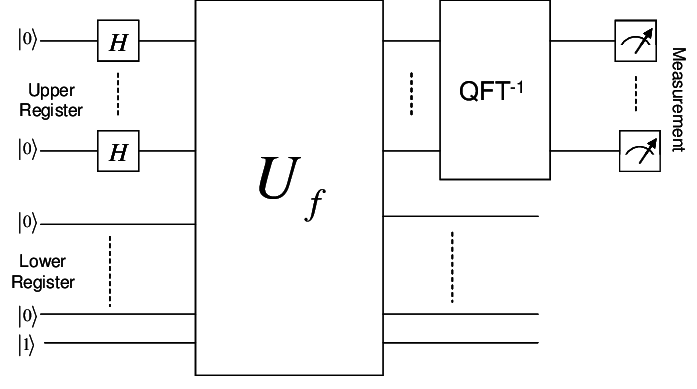
\includegraphics[scale=.5]{High-level-diagram-of-Shors-algorithm-Upper-register-consists-of-2n-qubits-and-holds}
    \centering
\end{figure}
\par Je potreba si vytvorit dva registry. Prvni registr pojmenuju jako kontrolni. Druhy jako cilovy.
Na velikost kontrolniho registru zalezei, jak moc je velka uspesnost dostat spravny vysledek a take jak moc presne vypocty budou.
Velikost ciloveho registru zvolime jako $n = log_2(N)$.
Pak velikost $2n$ bude dostacujici pro kontrolni registr.
\par Vsechny qubity z kontrolniho registru dame do stavu $0$. Vsechny qubity z ciloveho registru dame do stavu $0$ az na posledni qubit. Ten bude ve stavu 1.
Takze po inicializaci bude stav kvanotveho pocitace:
$$|\phi\rangle = |0\rangle^{\otimes 2n} |1\rangle$$ 
\par Dalsim krokem je potreba dostat kontrolni registr do superpozice pomoci Hadamard hradel:
$$|\phi_2\rangle = $$

\subsection{Implementace}
TODO

\newpage


\section{Zdroje}
\color{blue}
\fontsize{10pt}{0}
\url{https://cs.wikipedia.org/wiki/RSA}
\par\url{https://en.wikipedia.org/wiki/Shor%27s_algorithm}
\par\url{https://en.wikipedia.org/wiki/Quantum_logic_gate}
\par\url{https://arxiv.org/pdf/quant-ph/9508027.pdf}
\par\url{https://qiskit.org/}



\end{document}